\begin{uebsp}
\begin{Exercise}[label=ex:10.1]\index{Huffman-Code!Beispiel}\index{Huffman Algorithmus!Beispiel}
Bestimme für die Verteilung: 
\begin{align}
P = (0.1, 0.4, 0.05, 0.2, 0.25)
\end{align}
den Huffman-Code
\end{Exercise}
\begin{Answer}
Aufsteigend sortierte Verteilung:\\
P = (0.05, 0.1, 0.2, 0.25, 0.4)

    \item Fasse Knoten 0.05 und 0.1 zu einem neuen Knoten 0.15 zusammen:\\
\begin{center}
    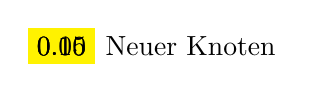
\begin{tikzpicture}[every tree node/.style={draw,circle},
       level distance=1.25cm,sibling distance=.5cm, anchor=west,
       edge from parent path={(\tikzparentnode) -- (\tikzchildnode)}]
        \Tree [.\node[fill=yellow,label=east: {Neuer Knoten}] (A) {0.15} ; 
        [.\node (B) {0.05}; ] [.\node (C) {0.10}; ] ]
    \end{tikzpicture}\\
\end{center}

Übrig bleibt die Menge: (0.15, 0.2, 0.25, 0.4)
\item Fasse Knoten 0.15 und 0.2 zusammen:\\
\begin{center}
    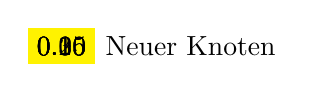
\begin{tikzpicture}[every tree node/.style={draw,circle},
       level distance=1.25cm,sibling distance=.5cm, anchor=west,
       edge from parent path={(\tikzparentnode) -- (\tikzchildnode)}]
        \Tree [.\node[fill=yellow,label=east: {Neuer Knoten}] (A) {0.35} ; 
        [.\node (B) {0.15}; 
            [.\node (D) {0.05}; ][.\node (E) {0.10}; ]
        ] [.\node (C) {0.20}; ] ]
    \end{tikzpicture}\\
\end{center}

Übrig bleibt die Menge: (0.25, 0.35, 0.4)
\item Fasse Knoten 0.25 und 0.35 zusammen:\\
\begin{center}
    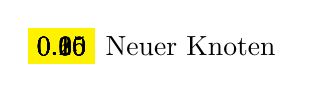
\begin{tikzpicture}[every tree node/.style={draw,circle},
       level distance=1.25cm,sibling distance=.5cm, anchor=west,
       edge from parent path={(\tikzparentnode) -- (\tikzchildnode)}]
        \Tree [.\node[fill=yellow,label=east: {Neuer Knoten}] (A) {0.60} ; 
        [.\node (B) {0.35}; 
            [.\node (D) {0.15}; 
                [.\node (F) {0.05}; ][.\node (G) {0.10}; ]
            ][.\node (E) {0.20}; ]
        ] [.\node (C) {0.25}; ] ]
    \end{tikzpicture}\\
\end{center}
Übrig bleibt die Menge: (0.4, 0.6)
\item Fasse Knoten 0.4 und 0.6 zusammen:\\
\begin{center}
    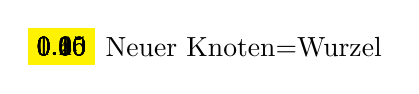
\begin{tikzpicture}[every tree node/.style={draw,circle},
       level distance=1.25cm,sibling distance=.5cm, anchor=west,
       edge from parent path={(\tikzparentnode) -- (\tikzchildnode)}]
        \Tree [.\node[fill=yellow,label=east: {Neuer Knoten=Wurzel}] (A) {1.00} ; 
        [.\node (B) {0.60}; 
            [.\node (D) {0.35}; 
                [.\node (F) {0.15}; 
                    [.\node (F) {0.05}; ][.\node (G) {0.10}; ]
                ][.\node (G) {0.20}; ]
            ][.\node (E) {0.25}; ]
        ] [.\node (C) {0.40}; ] ]
    \end{tikzpicture}\\
\end{center}Ergibt den fertigen Baum für den Huffman-Code.

\end{Answer}
\end{uebsp}
